%compare accuracy of the algorithms
%put global feature importance for each algorithm and compare them
%for the best algorithm, put feature importance for each region and compare them


\chapter{Results}

\section{Results of the Models}

\begin{table}[htbp]
    \centering
    \begin{tabular}{|l|c|c|}
    \hline
    \textbf{Model}           & \textbf{Accuracy} & \textbf{Weighted Average of Precision} \\ \hline
    Logistic Regression & 85.42\%          & 0.73                \\ \hline
    Decision Tree       & 75.97\%          & 0.77              \\ \hline
    Random Forests      & 85.67\%          & 0.83             \\ \hline
    Naïve Bayes         & 85.04\%          & 0.75               \\ \hline
    KNN                 & 83.92\%          & 0.80               \\ \hline
    \end{tabular}
    \caption{Accuracy and Weighted Average of Precision of Different Models}
    \end{table}
    
According to the results shown in the table above, Random Forests and Logistic Regression have the highest accuracy values. However, Random Forests has a
higher value on weighted Average of Precision
%what do you mean by "higher value on weighted Average of Precision"?
and if the confusion matrixes are compared it can be shown that Random Forests has a higher 
probability of making correct predictions. This makes Random Forests the best model for this dataset with 85.67\% accuracy. 
In general, all the models have high accuracy values, which indicates that the dataset is well-suited for classification. Even the worst model, Decision Tree, has an accuracy of 75.97\%, which is still a high value.\\
Furthermore, our accuracy results are better than the article studied for the literature, in which the best algorithm, Logistic Regression, had an accuracy of 52\%. This could be due to the fact that their dataset was smaller and less diverse than the dataset used in this study.
\\

\section{Global Feature Importance Analysis}

It's important to understand the global importance of the features in the dataset to be able to make better predictions.

The Random Forest model shows that globally many features are important for predicting the popularity of a song: \textit{tempo} is the most important, but also \textit{loudness}, \textit{duration}, \textit{acousticness}, \textit{speechiness}, \textit{valence}, \textit{danceability}, \textit{energy} and \textit{liveness} have similarly high values of importance. The least important features are \textit{instrumentalness}, \textit{key}, \textit{mode} and \textit{time signature}. These last two features were already shown to not be important in the correlation matrix.
On the other hand, all the other models show that 
\textit{dancebility} is the most important feature, with a significant difference from the other features.

This difference can be attributed to the inherent complexity and flexibility of the Random Forest
algorithm, which allows it to capture intricate patterns and interactions in the data that other models may not.\\
Also the literature supports the \textit{danceability} as the most important feature for predicting the popularity of a song, with a significant difference from the other features.\\




\newpage
\textbf{Global Feature Importance Extracted From Different Models:}
\begin{figure}[h]
    \centering
    \begin{minipage}{0.45\textwidth}
        \centering
        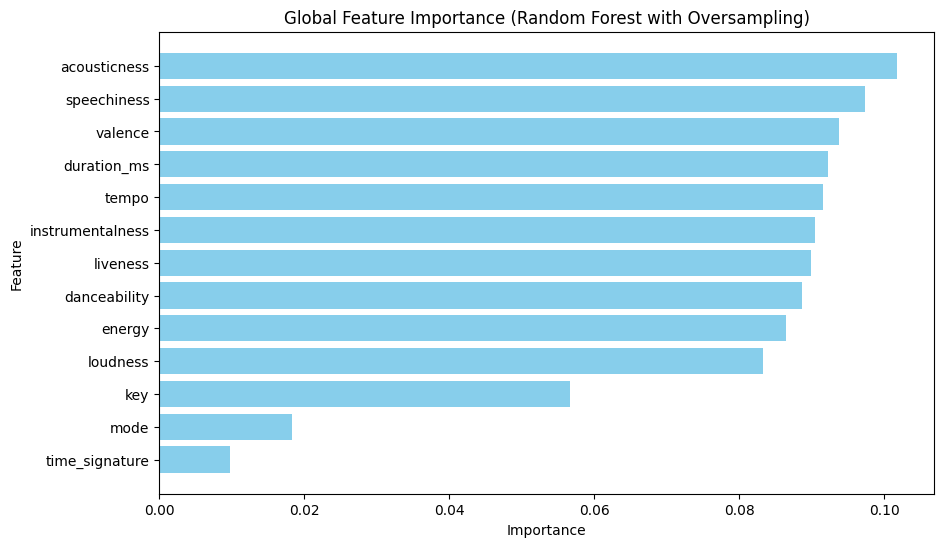
\includegraphics[width=\linewidth]{media/random_forest_feature_imp_global.png}
        \caption{Global Feature Importance Using Random Forests Model}
    \end{minipage}%
    \hspace{0.05\textwidth} % Space between the two figures
    \begin{minipage}{0.45\textwidth}
        \centering
        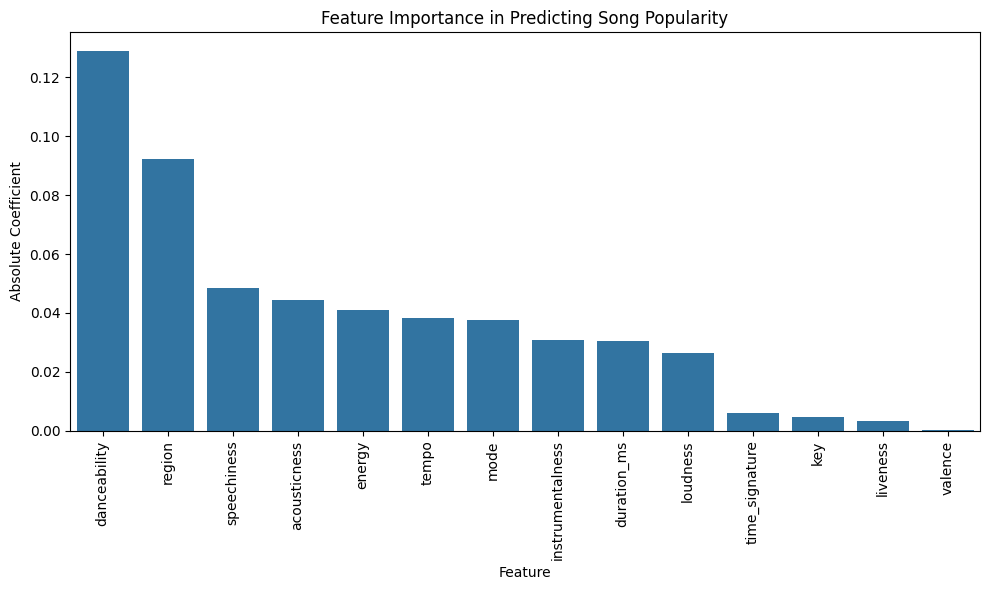
\includegraphics[width=\linewidth]{media/logistic_reg_feature_imp_global.png}
        \caption{Global Feature Importance Using Logistic Regression Model}
    \end{minipage}
\end{figure}
\begin{figure}[h]
    \centering
    \begin{minipage}{0.45\textwidth}
        \centering
        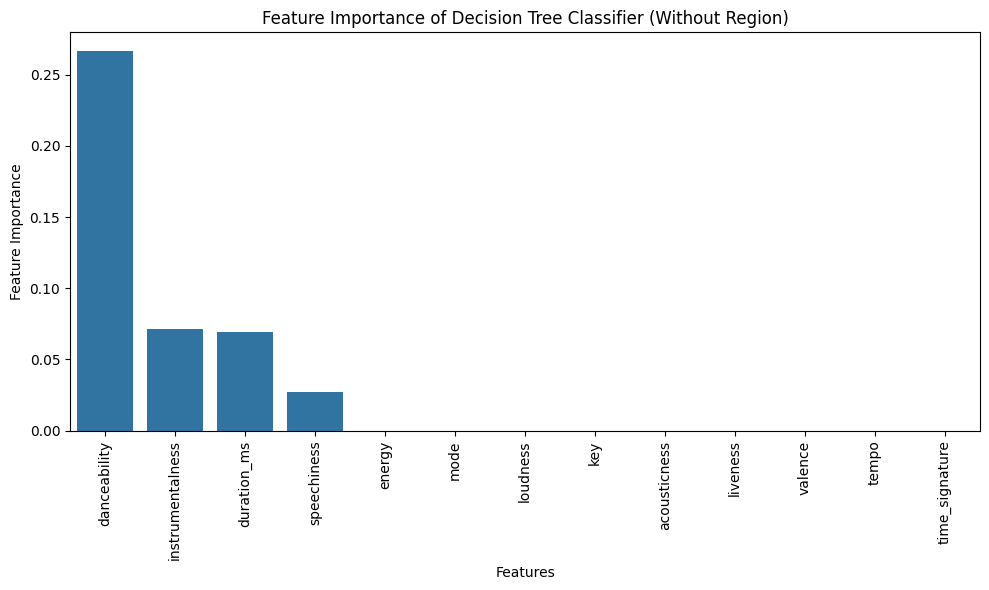
\includegraphics[width=\linewidth]{media/decision_tree_fea_imp_global.png}
        \caption{Global Feature Importance Using Decision Tree Model}
    \end{minipage}%
    \hspace{0.05\textwidth} % Space between the two figures
    \begin{minipage}{0.45\textwidth}
        \centering
        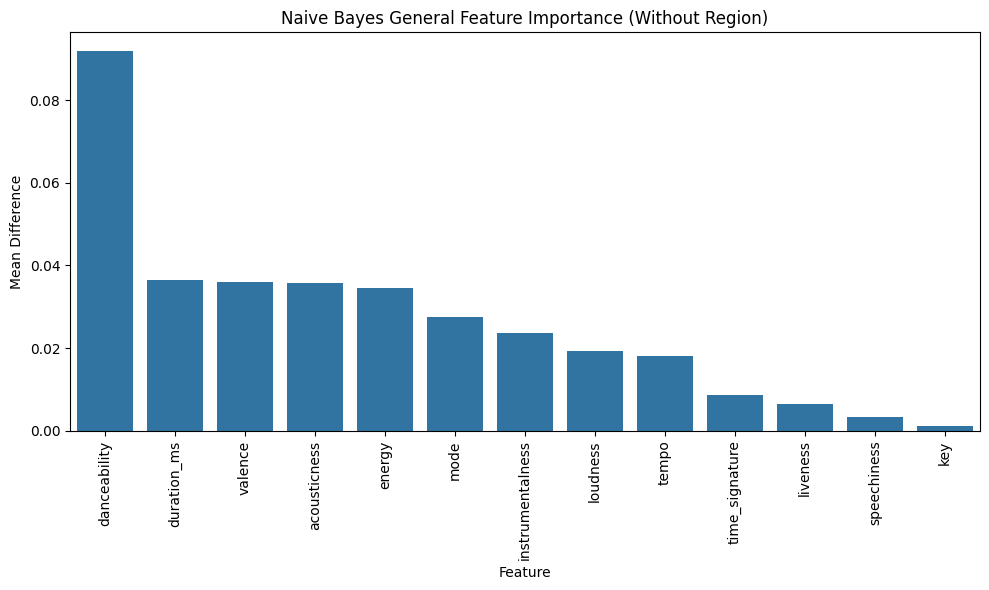
\includegraphics[width=\linewidth]{media/naive_bayes_fea_imp_global.png}
        \caption{Global Feature Importance Using Naïve Bayes Model}
    \end{minipage}
\end{figure}

\newpage

\section{Regional Feature Importance Analysis}


The feature importance is extracted not only globally but also for each region. To do that we decide to consider the Random Forest model as the best model.
This analysis helps to understand how the music tastes of different regions are shaped by audio features.
The most important features for each region are shown below. The mean values of these features are also given to help understand the music tastes of each region.

%NB: These graphs also show the region column, it's a waste of space, we should remove it

\textbf{Feature Importance for Each Region Extracted From Random Forest Model:}
\begin{figure}[h]
    \centering
    \begin{minipage}{0.45\textwidth}
        \centering
        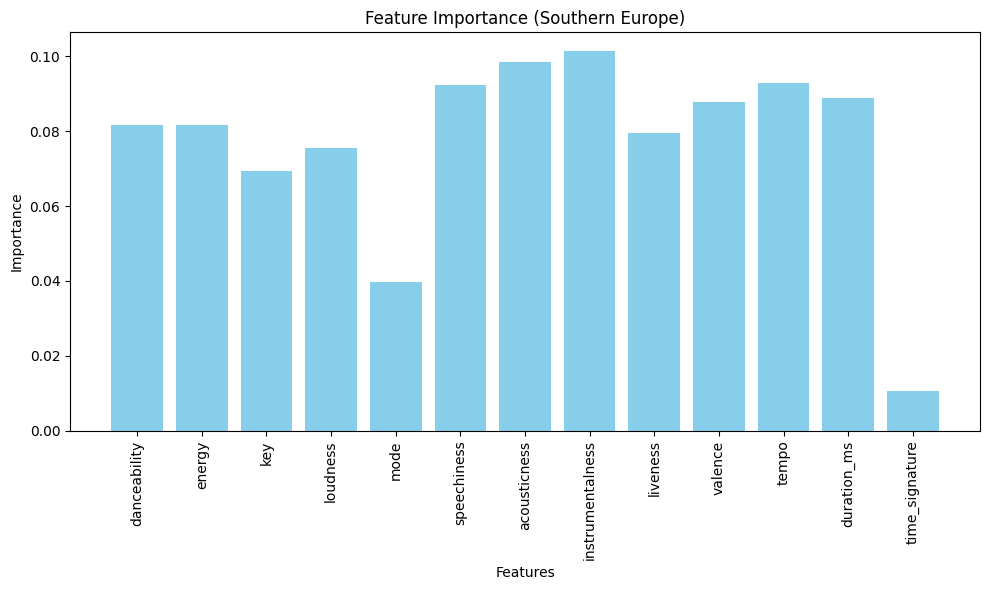
\includegraphics[width=\linewidth]{media/rf_feature_imp_northen_europe.png}
        \caption{Feature Importance in North Europe}
    \end{minipage}%
    \hspace{0.05\textwidth} % Space between the two figures
    \begin{minipage}{0.45\textwidth}
        \centering
        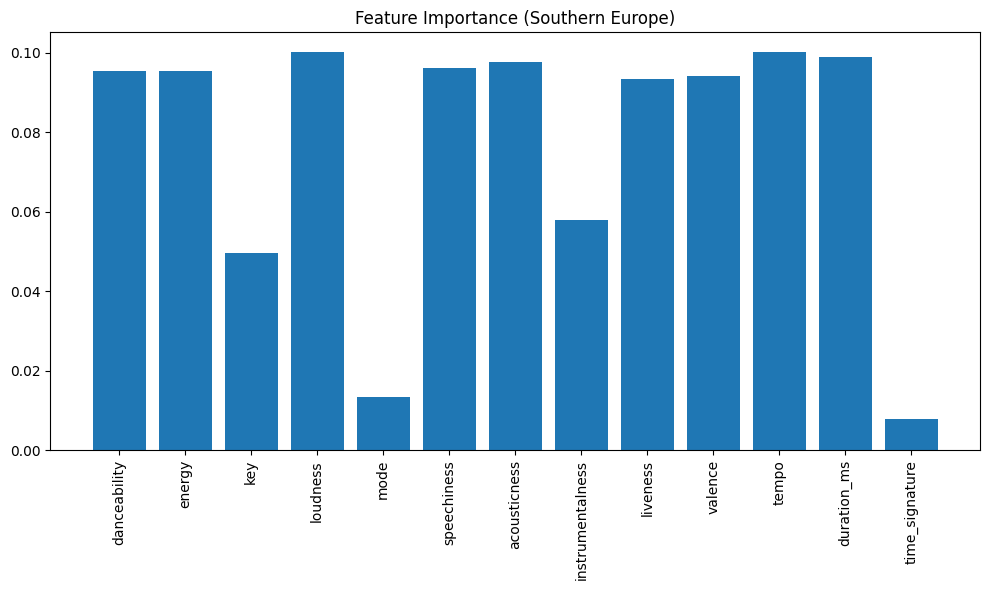
\includegraphics[width=\linewidth]{media/rf_feature_imp_southern_europe.png}
        \caption{Feature Importance in South Europe}
    \end{minipage}
\end{figure}
\begin{figure}[h]
    \centering
    \begin{minipage}{0.45\textwidth}
        \centering
        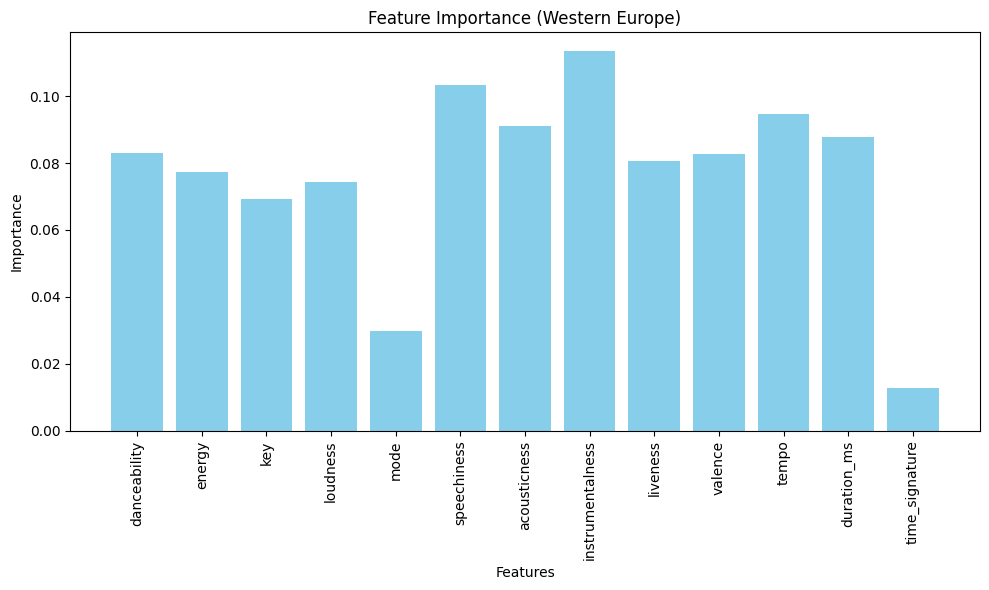
\includegraphics[width=\linewidth]{media/rf_feature_imp_western_europe.png}
        \caption{Feature Importance in Western Europe}
    \end{minipage}%
    \hspace{0.05\textwidth} % Space between the two figures
    \begin{minipage}{0.45\textwidth}
        \centering
        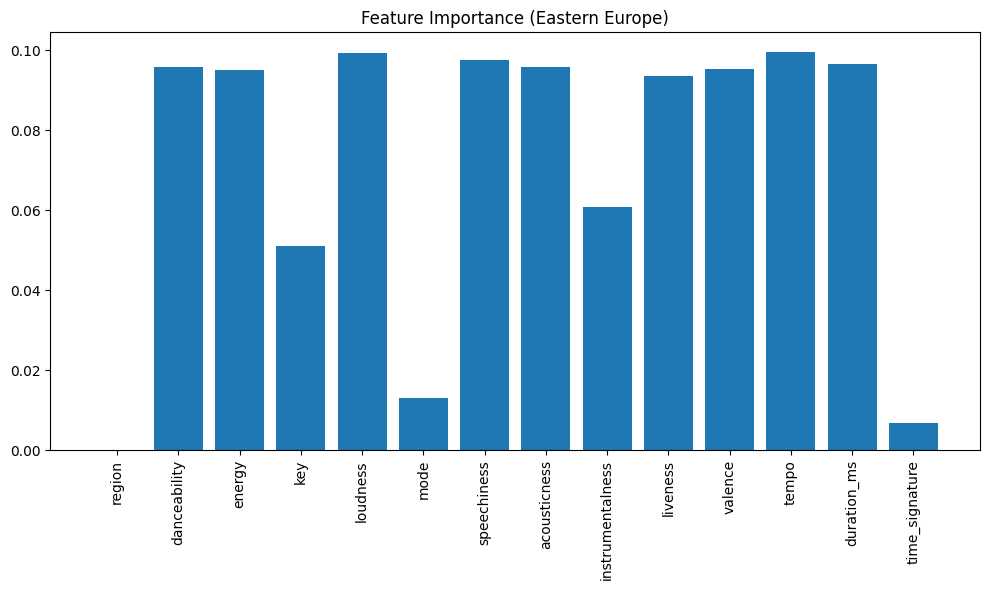
\includegraphics[width=\linewidth]{media/rf_feature_imp_eastern_europe.png}
        \caption{Feature Importance in Eastern Europe}
    \end{minipage}
\end{figure}
\begin{figure}[h]
    \centering
    \begin{minipage}{0.45\textwidth}
        \centering
        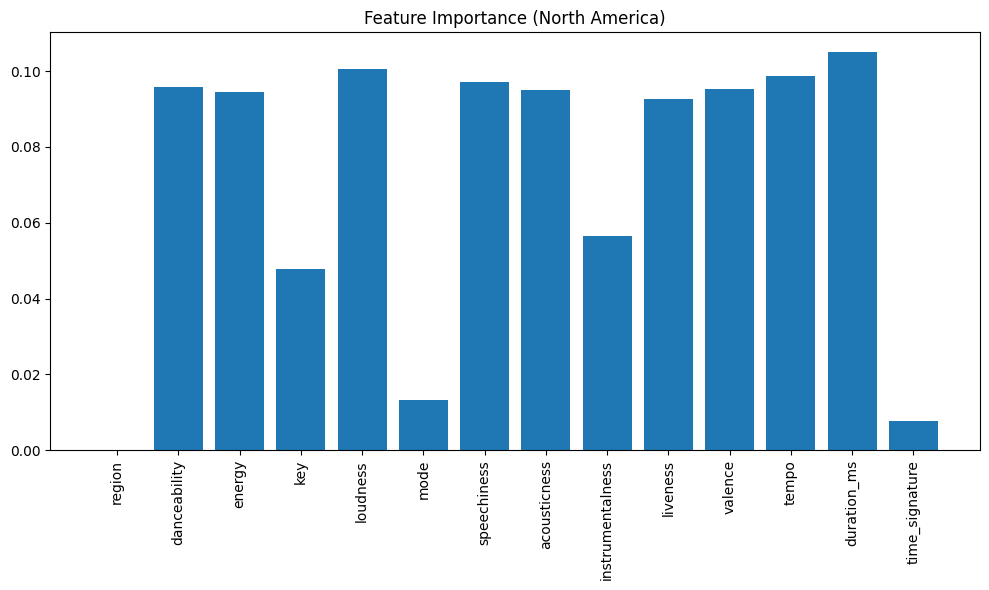
\includegraphics[width=\linewidth]{media/rf_feature_imp_north_america.png}
        \caption{Feature Importance in North America}
    \end{minipage}%
    \hspace{0.05\textwidth} % Space between the two figures
    \begin{minipage}{0.45\textwidth}
        \centering
        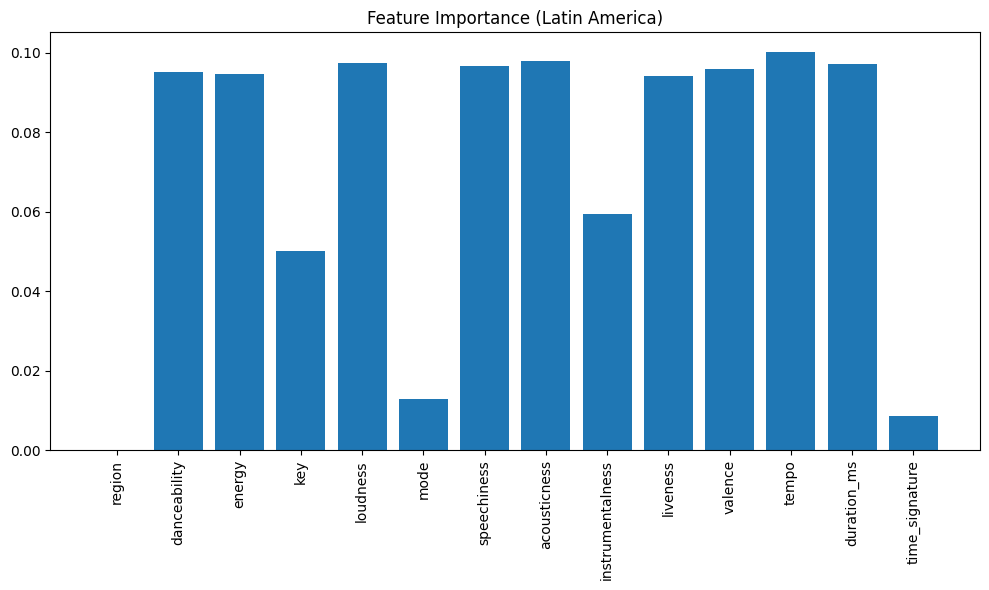
\includegraphics[width=\linewidth]{media/rf_feature_imp_latin_america.png}
        \caption{Feature Importance in Latin America}
    \end{minipage}
\end{figure}
\begin{figure}[h]
    \centering
    \begin{minipage}{0.45\textwidth}
        \centering
        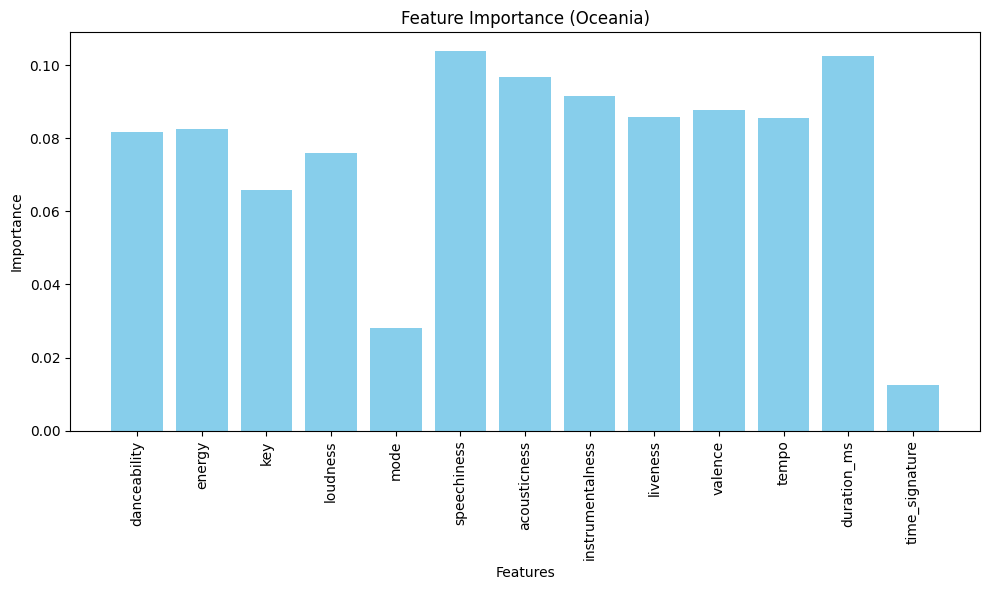
\includegraphics[width=\linewidth]{media/rf_feature_imp_ocenia.png}
        \caption{Feature Importance in Oceania}
    \end{minipage}%
    \hspace{0.05\textwidth} % Space between the two figures
    \begin{minipage}{0.45\textwidth}
        \centering
        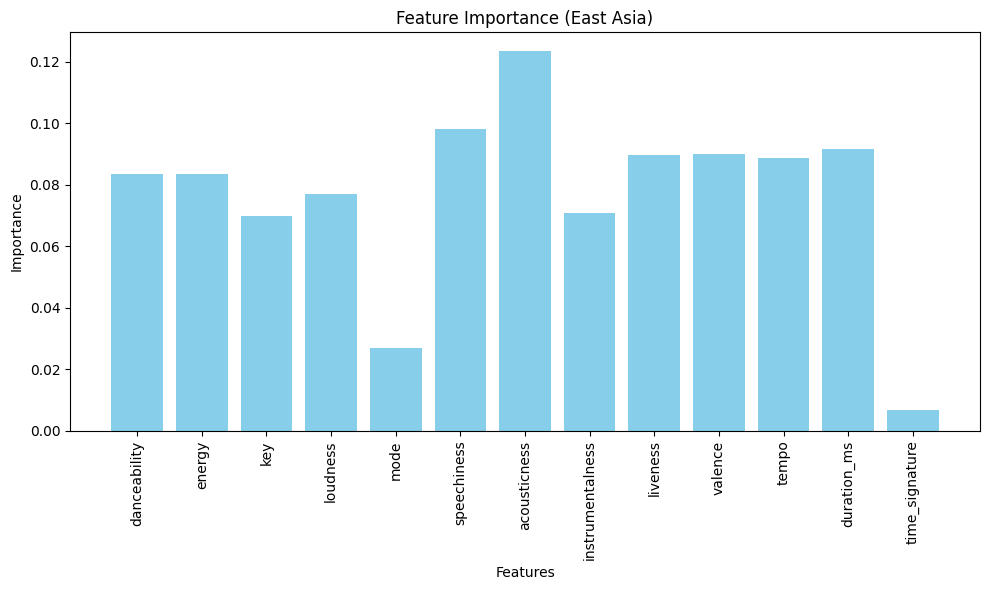
\includegraphics[width=\linewidth]{media/rf_feature_imp_east_asia.png}
        \caption{Feature Importance in East Asia}
    \end{minipage}
\end{figure}
\begin{figure}[h]
    \centering
    \begin{minipage}{0.45\textwidth}
        \centering
        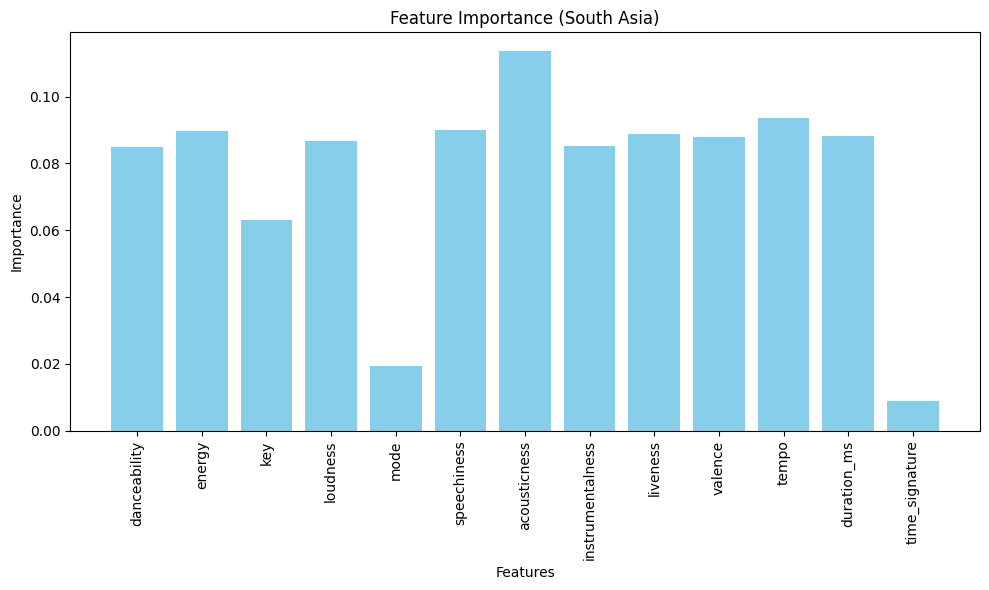
\includegraphics[width=\linewidth]{media/rf_feature_imp_south_asia.png}
        \caption{Feature Importance in South Asia}
    \end{minipage}%
    \hspace{0.05\textwidth} % Space between the two figures
    \begin{minipage}{0.45\textwidth}
        \centering
        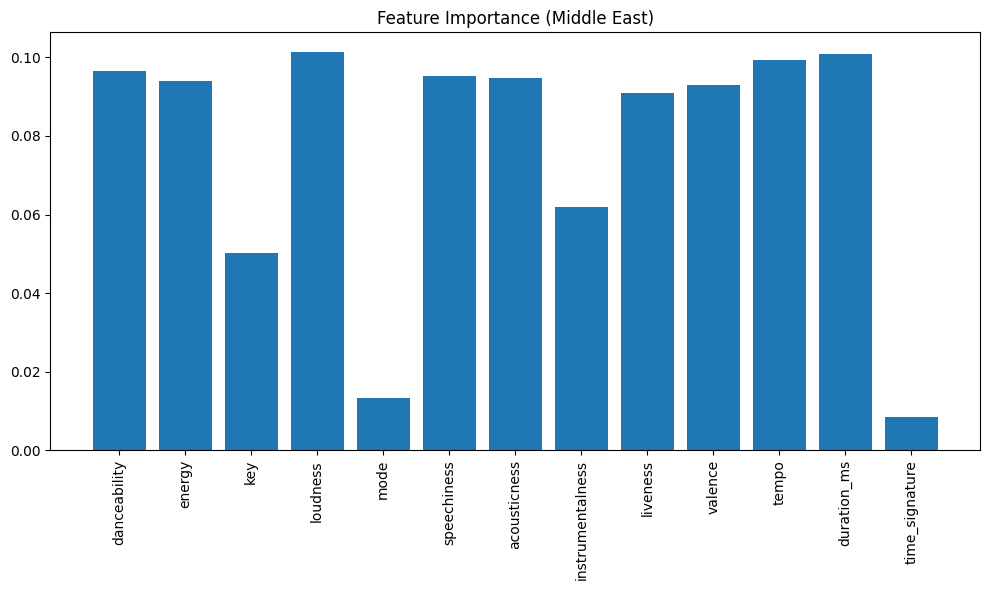
\includegraphics[width=\linewidth]{media/rf_feature_imp_middle_east.png}
        \caption{Feature Importance in Middle East}
    \end{minipage}
\end{figure}
\begin{figure}[h]
    \centering
    \begin{minipage}{0.45\textwidth}
        \centering
        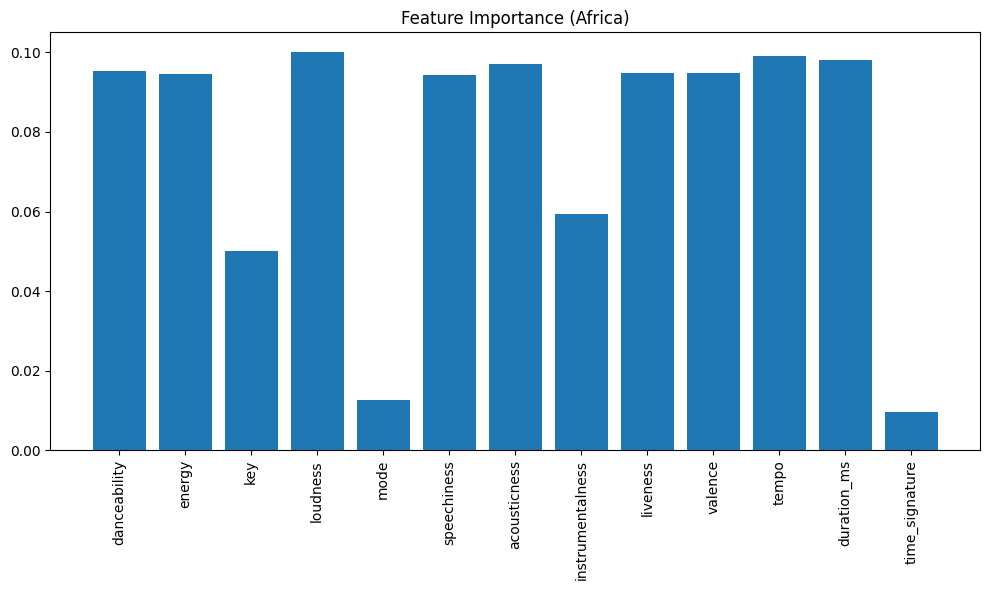
\includegraphics[width=\linewidth]{media/rf_feature_imp_africa.png}
        \caption{Feature Importance in Africa}
    \end{minipage}
\end{figure}

\clearpage 

\subsection{Important Features for Each Region and Their Mean Values}

Generally, the different regions tend to have a coherence in the importance of the features. For example, \textit{tempo} and \textit{loudness} are among the top 5 important features in all regions. \\



\textbf{Northern Europe}
\begin{enumerate}
    \item \textbf{Duration\_ms}: Importance: 0.1021, Mean Value: 203514.75
    \item \textbf{Loudness}: Importance: 0.0995, Mean Value: -7.35
    \item \textbf{Tempo}: Importance: 0.0972, Mean Value: 121.29
    \item \textbf{Danceability}: Importance: 0.0965, Mean Value: 0.64
    \item \textbf{Acousticness}: Importance: 0.0963, Mean Value: 0.23
\end{enumerate}

\textbf{Southern Europe}
\begin{enumerate}
    \item \textbf{Loudness}: Importance: 0.1012, Mean Value: -7.02
    \item \textbf{Duration\_ms}: Importance: 0.0996, Mean Value: 210862.34
    \item \textbf{Tempo}: Importance: 0.0986, Mean Value: 121.24
    \item \textbf{Speechiness}: Importance: 0.0968, Mean Value: 0.12
    \item \textbf{Acousticness}: Importance: 0.0965, Mean Value: 0.27
\end{enumerate}

\textbf{Western Europe}
\begin{enumerate}
    \item \textbf{Loudness}: Importance: 0.1006, Mean Value: -7.26
    \item \textbf{Tempo}: Importance: 0.1004, Mean Value: 120.90
    \item \textbf{Duration\_ms}: Importance: 0.0990, Mean Value: 205864.40
    \item \textbf{Acousticness}: Importance: 0.0965, Mean Value: 0.25
    \item \textbf{Speechiness}: Importance: 0.0960, Mean Value: 0.15
\end{enumerate}

\textbf{Eastern Europe}
\begin{enumerate}
    \item \textbf{Tempo}: Importance: 0.0995, Mean Value: 122.33
    \item \textbf{Loudness}: Importance: 0.0993, Mean Value: -7.34
    \item \textbf{Speechiness}: Importance: 0.0975, Mean Value: 0.13
    \item \textbf{Duration\_ms}: Importance: 0.0966, Mean Value: 205515.98
    \item \textbf{Acousticness}: Importance: 0.0959, Mean Value: 0.24
\end{enumerate}

\textbf{North America}
\begin{enumerate}
    \item \textbf{Duration\_ms}: Importance: 0.1050, Mean Value: 206987.98
    \item \textbf{Loudness}: Importance: 0.1005, Mean Value: -6.99
    \item \textbf{Tempo}: Importance: 0.0988, Mean Value: 121.36
    \item \textbf{Speechiness}: Importance: 0.0972, Mean Value: 0.13
    \item \textbf{Danceability}: Importance: 0.0958, Mean Value: 0.66
\end{enumerate}


\textbf{Latin America}
\begin{enumerate}
    \item \textbf{Tempo}: Importance: 0.1001, Mean Value: 122.61
    \item \textbf{Acousticness}: Importance: 0.0979, Mean Value: 0.29
    \item \textbf{Loudness}: Importance: 0.0974, Mean Value: -6.71
    \item \textbf{Duration\_ms}: Importance: 0.0972, Mean Value: 217127.50
    \item \textbf{Speechiness}: Importance: 0.0965, Mean Value: 0.11
\end{enumerate}

\textbf{Oceania}
\begin{enumerate}
    \item \textbf{Duration\_ms}: Importance: 0.1061, Mean Value: 213396.98
    \item \textbf{Tempo}: Importance: 0.0986, Mean Value: 120.82
    \item \textbf{Danceability}: Importance: 0.0981, Mean Value: 0.65
    \item \textbf{Loudness}: Importance: 0.0977, Mean Value: -7.05
    \item \textbf{Acousticness}: Importance: 0.0962, Mean Value: 0.23
\end{enumerate}

\textbf{East Asia}
\begin{enumerate}
    \item \textbf{Tempo}: Importance: 0.1027, Mean Value: 121.52
    \item \textbf{Duration\_ms}: Importance: 0.1005, Mean Value: 229571.73
    \item \textbf{Loudness}: Importance: 0.1004, Mean Value: -6.86
    \item \textbf{Acousticness}: Importance: 0.0986, Mean Value: 0.30
    \item \textbf{Speechiness}: Importance: 0.0967, Mean Value: 0.08
\end{enumerate}

\textbf{South Asia}
\begin{enumerate}
    \item \textbf{Loudness}: Importance: 0.1010, Mean Value: -7.39
    \item \textbf{Duration\_ms}: Importance: 0.1006, Mean Value: 222230.31
    \item \textbf{Tempo}: Importance: 0.0982, Mean Value: 119.92
    \item \textbf{Acousticness}: Importance: 0.0981, Mean Value: 0.36
    \item \textbf{Danceability}: Importance: 0.0960, Mean Value: 0.62
\end{enumerate}


\textbf{Middle East}
\begin{enumerate}
    \item \textbf{Duration\_ms}: Importance: 0.1019, Mean Value: 213894.57
    \item \textbf{Loudness}: Importance: 0.0988, Mean Value: -7.63
    \item \textbf{Tempo}: Importance: 0.0976, Mean Value: 120.14
    \item \textbf{Acousticness}: Importance: 0.0961, Mean Value: 0.30
    \item \textbf{Danceability}: Importance: 0.0954, Mean Value: 0.64
\end{enumerate}


\textbf{Africa}
\begin{enumerate}
    \item \textbf{Loudness}: Importance: 0.0992, Mean Value: -7.61
    \item \textbf{Tempo}: Importance: 0.0987, Mean Value: 120.41
    \item \textbf{Duration\_ms}: Importance: 0.0976, Mean Value: 219551.52
    \item \textbf{Acousticness}: Importance: 0.0963, Mean Value: 0.26
    \item \textbf{Liveness}: Importance: 0.0962, Mean Value: 0.17
\end{enumerate}

\newpage
\subsection{Interpretation of the Results}
\begin{itemize}
    \item\textbf{Tempo Variation}
    
While tempo is among the top 5 most important features in all regions, there is a clear variation in its mean values:
The highest tempo is in \textbf{Latin America} (122.61), while the lowest is in \textbf{South Asia} (119.92).
This suggests that Latin American music tends to have a slightly faster rhythm compared to South Asian music. These differences could reflect the regions' cultural preferences for more energetic or relaxed musical styles.
\item\textbf{Loudness Preferences}

Loudness is another common feature across all regions, yet it shows notable differences in mean values:
For instance, \textbf{North America} (-6.99) and \textbf{Latin America} (-6.71) tend to prefer louder music compared to regions like \textbf{Eastern Europe}(-7.34) and \textbf{South Asia} (-7.39).
These differences could indicate varying preferences for more dynamic or intense sound production, with North and Latin America leaning toward more "in-your-face" soundscapes, while regions like Eastern Europe and South Asia favor softer or more subdued sound levels.
\item\textbf{Regional Focus on Danceability}

Danceability is present in the top 5 important features in five regions: \textbf{Middle East}, \textbf{North America}, \textbf{Northern Europe}, \textbf{Oceania}, and \textbf{South Asia}.
This suggests that these regions emphasize the rhythmic elements of music that facilitate dancing, perhaps reflecting a stronger cultural or social inclination towards dance-centric activities. Regions like \textbf{Eastern Europe} or \textbf{East Asia}, where danceability is not in the top 5, may prioritize other aspects of music like lyrical content or acoustic richness.
\item\textbf{Acousticness Differences}

Acousticness, which measures the likelihood of a track being acoustic, shows varying importance across regions:
\textbf{South Asia} has a relatively high mean acousticness (0.36), while \textbf{Latin America} and \textbf{Oceania} have lower values (0.29 and 0.23 respectively).
This could indicate a stronger preference for traditional, organic instruments in South Asia, whereas Latin America and Oceania might favor more synthesized or electronic soundscapes.
\item\textbf{Speechiness and Spoken Elements}

Speechiness is featured in several regions, but the mean values show regional differences in how much spoken word is present in music:
For instance, \textbf{Latin America} (0.11) and \textbf{East Asia} (0.08) have lower speechiness compared to \textbf{Eastern Europe} (0.13) and \textbf{North America} (0.13).
This variation may reflect differing musical traditions: regions with lower speechiness may prefer more melodic, sung vocals, while those with higher values could incorporate more rap or spoken word elements.
\item\textbf{Duration of Tracks}

The duration\_ms of tracks also varies across regions:
\textbf{East Asia} has the longest average duration (229571.73 ms), while \textbf{Northern Europe} has shorter tracks (203514.75 ms).
Longer tracks in East Asia may suggest a preference for more complex or drawn-out compositions, while shorter tracks in Northern Europe may reflect a preference for more concise and easily consumable music.
\item\textbf{Regional Absence of Energy and Valence}

Surprisingly, energy and valence (happiness or emotional positivity) are absent from the top 5 important features in all regions.
This suggests that, although energy and valence are often associated with the overall feel or mood of a track, they are not as influential in shaping regional music preferences as tempo, loudness, or other features like acousticness or danceability. It could mean that other characteristics are more decisive in defining regional music tastes.
\item\textbf{Cultural and Historical Contexts}

The preferences for certain features (like acousticness in \textbf{South Asia} or danceability in \textbf{Oceania}) could be influenced by regional cultural contexts:
South Asia's higher acousticness might reflect a deeper connection to traditional, acoustic music forms like classical or folk music.
Oceania’s preference for danceability could be tied to its strong tradition of social and communal dance, particularly in Pacific Island cultures.
\item\textbf{Impact of Globalization}

The fact that features like tempo and loudness are consistently important across all regions may indicate a certain degree of global musical homogenization due to the influence of global pop and electronic music.
However, the variation in mean values suggests that, despite global influences, regional music cultures maintain distinct preferences and characteristics.
\item\textbf{Evolution of Regional Music Preferences}

Over time, these differences in preferences might evolve as global trends influence local tastes, or as regions increasingly revert to traditional forms in response to external influences.
Monitoring how these values change over time could offer insights into the trajectory of regional music trends.
These considerations highlight the diversity in music preferences across regions, while also emphasizing certain universal elements that transcend cultural boundaries. Understanding these nuances helps map out how cultural and social factors influence regional music trends.
\end{itemize}
